\documentclass[14pt]{article}
\usepackage[utf8]{inputenc}
\usepackage[T1]{fontenc}
\usepackage{graphicx}
\usepackage{float}

\title{Rapport projet Calcul Parallèle}
\author{Naïm ALI-MOUSSA}
\date{}

\begin{document}

\maketitle

\newpage

\section*{Table des sommaires}
\tableofcontents

\newpage
\section{Introduction}
L'objectif de ce projet est d'implanter les produits \textit{Matrice * Vecteur}, \textit{Vecteur * Matrice} et \textit{Matrice * Matrice}. Pour cela, nous développerons notre programme en langage C.\\
Dans un premier temps, nous aborderons ces opérations de manière séquentielle. Nous testerons les différents types offerts par le langage C, comparerons les performances entre les opérations, mesurerons le nombre de cycles CPU nécessaires à leur exécution selon différentes implémentations, et utiliserons des options d'optimisation du compilateur \texttt{gcc} ainsi que diverses autres techniques.\\
Dans un second temps, nous implémenterons ces calculs selon une approche SIMD à l'aide des instructions \textbf{AVX2}, afin de paralléliser les traitements et de mesurer les gains de performance obtenus par rapport à la version séquentielle.\\
Pour ne pas disperser l'analyse au vu des nombreuses configurations possibles on va seulement se concentrer sur la comparaison de ces opérations en gardant le même type, c'est-à-dire le type \textbf{int64t} et constater les différences avec diverses méthodes.

\newpage
\section{Architecture du projet}
Pour réaliser efficacement ce projet il faut mettre en place une architecture propre et organisée.\\
Je vais opter de façon classique pour des projets réalisées en C en utilisant un \textbf{Makefile} afin de pouvoir compiler beaucoup plus facilement et gérer mes différents fichiers. De plus j'aurai plusieurs fichiers sources avec leurs équivalents en header qui contiendra les librairies nécessaires pour réaliser les fonctions dans les fichiers.c.\\
Le fichier \textbf{global.h} est celui qui contient toutes les librairies comme: stdio.h, stlib.h, etc. Cela sera utile afin d'éviter des dépendances cycliques et que cela engendre des problèmes à la compilation.\\
Le fichier \textbf{ccount.h} contient les macros pour pouvoir mesurer les temps CPU avec l'algorithme de mesures de performances qui est énoncé dans le cours.

\newpage
\section{Les représentations de matrice en séquentielle}
\subsection{Tableau à 1 dimension}
La première méthode implémentée a été de créer des matrices à 1 seule dimension, ils seront représentés par des pointeurs sur \texttt{int64t*}. Voici un graphique qui va pouvoir afficher les différences de nombres de cycles CPU entre ces 3 opérations:
\begin{figure}[h!]
    \centering
    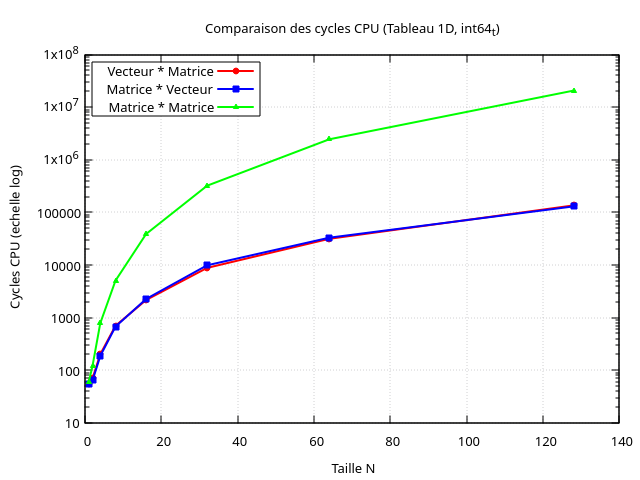
\includegraphics[width=0.85\textwidth]{courbe0_tab_1D.png}
    \caption{Comparaison du nombre de cycles CPU pour les trois opérations (tableau 1D) sans optimisation \texttt{-O0}.}
    \label{fig:courbe_1d}
\end{figure}

Les mesures du nombre de cycles CPU ont été effectuées avec les fonctions \texttt{mesure\_vec\_mat}, \texttt{mesure\_mat\_vec} et \texttt{mesure\_mat\_mat}, en faisant varier la constante $N$ de $2^1$ à $2^7$ (en multipliant $N$ par $2$ à chaque étape).
À première vue, l'opération \textit{Matrice $\times$ Matrice} est beaucoup plus coûteuse en cycles CPU que les deux autres. Ce résultat est tout à fait cohérent avec la complexité algorithmique et le volume de données manipulé :
\begin{itemize}
    \item \textbf{Complexité temporelle :} Le produit matriciel repose sur trois boucles imbriquées ($i$, $j$ et $k$, où $i$ parcourt les lignes de la matrice de gauche, $j$ les colonnes de la matrice de droite et $k$ l'indice commun), ce qui donne une complexité en $O(N^3)$. À l'inverse, les produits \textit{Matrice $\times$ Vecteur} et \textit{Vecteur $\times$ Matrice} ne nécessitent que deux boucles imbriquées, soit une complexité quadratique en $O(N^2)$ (parce que les matrices et vecteurs partageant la même dimension $N$).
    \item \textbf{Volume de données en mémoire :} Le produit matriciel manipule deux matrices carrées, soit $2N^2$ éléments en mémoire, contre $N^2 + N$ éléments pour les opérations impliquant un vecteur.
\end{itemize}
Ainsi, le produit matriciel effectue $N$ fois plus d'opérations élémentaires que les deux autres produits ($N^3$ contre $N^2$), ce qui explique l'écart important observé sur le nombre de cycles CPU dès que $N$ augmente.
\\
\\
En comparant plus précisément les deux opérations en $O(N^2)$ sans optimisation (\texttt{-O0}), on observe que \textit{Matrice $\times$ Vecteur} est légèrement plus lent que \textit{Vecteur $\times$ Matrice} pour les petites tailles ($N \le 64$), puis reprend l'avantage en étant un peu plus rapide à partir de $N = 128$.

Ce phénomène s'explique par deux facteurs complémentaires :
\begin{itemize}
    \item \textbf{Absence d'allocation dans les registres :} D'après le manuel de \texttt{gcc} (\texttt{man gcc}), l'option \texttt{-O0} vise à réduire le temps de compilation et à produire les résultats attendus lors du débogage. Concrètement, le compilateur n'applique aucune optimisation sur le code généré : les variables restent allouées en mémoire sur la pile plutôt que dans les registres CPU et aucune boucle n'est transformée, ce qui explique les temps d'exécution élevés observés sur cette première courbe. À chaque itération de la boucle interne, les variables locales et les calculs d'indices (\texttt{i * N + j}) sont systématiquement lus et réécrits sur la pile en mémoire, générant un surcoût d'instructions CPU qui masque l'effet du cache tant que $N \le 64$.

    \item \textbf{Saturation du cache L1 et localité spatiale à $N = 128$ :} Pour accélérer les accès mémoire par rapport à la RAM, le processeur dispose d'une hiérarchie de mémoires caches (L1, L2, L3). Le cache de données de niveau 1 (L1) est le plus rapide mais aussi le plus petit (généralement $32$~Ko ou $48$~Ko). Lorsque $N = 128$, la matrice contient $128 \times 128 = 16\,384$ éléments de type \texttt{int64\_t} ($8$~octets chacun), soit un volume de $128$~Ko qui dépasse la capacité du cache L1. Cela entraîne des défauts de cache (\textit{cache misses}) vers les niveaux L2 et L3. La matrice étant stockée de manière contiguë ligne par ligne, \textit{Matrice $\times$ Vecteur} parcourt les éléments consécutivement et profite directement des $8$ éléments chargés simultanément dans chaque ligne de cache de $64$~octets, tandis que \textit{Vecteur $\times$ Matrice} effectue des sauts de $N$ éléments en mémoire, ce qui multiplie les défauts de cache L1 et explique que \textit{Matrice $\times$ Vecteur} repasse devant à $N = 128$.
\end{itemize}

Cette différence d'accès mémoire s'explique directement par la notion de \textit{stride}, qui désigne la distance en mémoire entre deux valeurs consécutivement accédées. \textit{Matrice $\times$ Vecteur} possède un \textit{stride} de $1$, tandis que \textit{Vecteur $\times$ Matrice} possède un \textit{stride} de $N$ : combiné à la saturation du cache L1, ce pas d'accès élevé pénalise directement cette seconde méthode dès que la taille des données augmente.
\\\\
Et voici un autre graphique mais cette fois-ci optimisée:

\begin{figure}[h!]
    \centering
    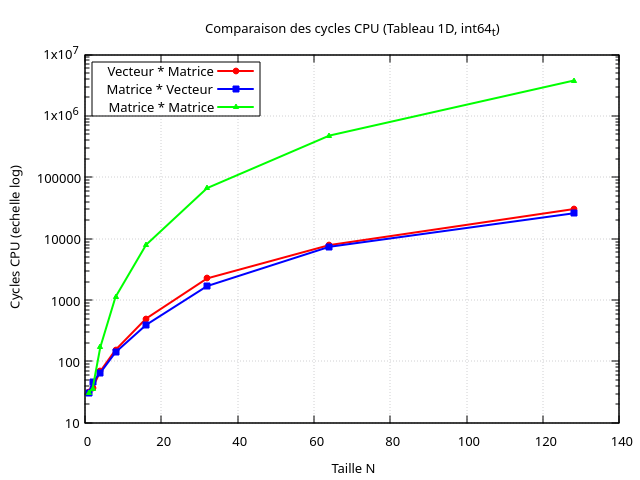
\includegraphics[width=0.85\textwidth]{courbe02_tab_1D.png}
    \caption{Comparaison du nombre de cycles CPU pour les trois opérations (tableau 1D) avec optimisation \texttt{-O2}.}
    \label{fig:courbe_1d}
\end{figure}

On constate globalement la même hiérarchie entre les opérations, sauf qu'avec \texttt{-O2}, le nombre de cycles CPU chute fortement et \textit{Matrice $\times$ Vecteur} est désormais  plus rapide que \textit{Vecteur $\times$ Matrice} pour toutes les valeurs de $N$.
\\
En effet, dans \textit{Matrice $\times$ Vecteur}, la matrice (opérande de gauche, stockée de manière contiguë dans un tableau 1D \texttt{int64\_t*}) est parcourue ligne par ligne, tandis que dans \textit{Vecteur $\times$ Matrice} (matrice à droite), elle est parcourue colonne par colonne. La différence de temps d'exécution s'explique alors par l'interaction entre le compilateur et la mémoire :

\begin{itemize}
    \item \textbf{Effet de l'optimisation avec \texttt{-O2} :} D'après le manuel de \texttt{gcc} (\texttt{man gcc}), l'option \texttt{-O2} applique la quasi-totalité des optimisations n'impliquant pas de compromis entre l'espace mémoire et la vitesse d'exécution. Contrairement à \texttt{-O0}, cette option augmente le temps de compilation mais améliore nettement les performances du code généré en activant notamment :
    \begin{itemize}
        \item \textbf{Élimination du surcoût CPU :} le compilateur place les variables dans les registres, factorise les calculs d'adresses redondants ($i \times N$) hors des boucles (\texttt{-fgcse}, \texttt{-ftree-pre}) et réordonne les instructions (\texttt{-fschedule-insns}) pour limiter les temps d'attente ;
        \item \textbf{Vectorisation prudente :} il active l'auto-vectorisation (\texttt{-ftree-loop-vectorize}), mais la bride avec un modèle de coût conservateur (\texttt{-fvect-cost-model=very-cheap}) qui ne réorganise pas l'ordre des boucles.
    \end{itemize}
    \item \textbf{L'accès mémoire comme facteur limitant :} Le processeur n'étant plus freiné par des instructions redondantes ni par des accès constants à la pile, la vitesse d'accès aux données devient déterminante. Comme établi précédemment, le parcours ligne par ligne de \textit{Matrice $\times$ Vecteur} bénéficie d'un \textit{stride} de $1$ (exploite pleinement les lignes de cache de $64$~octets), tandis que le parcours colonne par colonne de \textit{Vecteur $\times$ Matrice} impose un \textit{stride} de $N$, multipliant les défauts de cache dès que $N \ge 8$.
\end{itemize}

Ceci explique pourquoi, dès l'activation de \texttt{-O2}, \textit{Matrice $\times$ Vecteur} est plus rapide que \textit{Vecteur $\times$ Matrice} sur l'ensemble de la courbe.
\\\\
Puis une dernière observation se fait en observant la courbe avec une autre méthode d'optimisation.

\begin{figure}[h!]
    \centering
    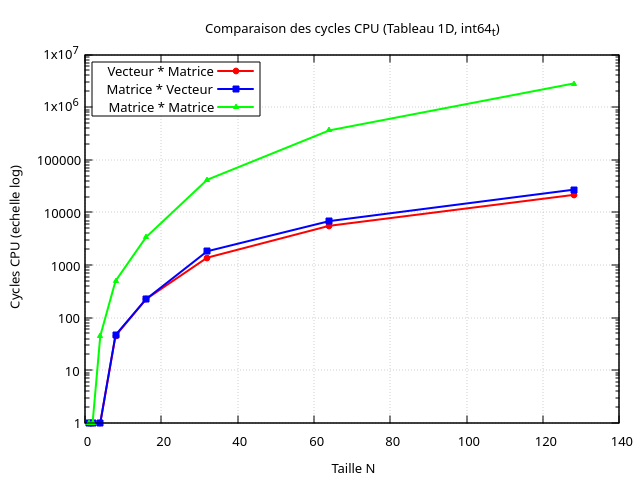
\includegraphics[width=0.85\textwidth]{courbefast_tab1D.png}
    \caption{Comparaison du nombre de cycles CPU pour les trois opérations (tableau 1D) avec optimisation \texttt{-Ofast}.}
    \label{fig:courbe_1d}
\end{figure}

On constate cette fois-ci que c'est l'inverse que ce qui se passait avec l'option \textit{-Ofast}, que dans cet exemple c'est \textit{Matrice $\times$ Vecteur} qui est moins rapide que \textit{Vecteur $\times$ Matrice} sur l'ensemble de la courbe. 
\\
D'après le manuel de \texttt{gcc} (\texttt{man gcc}), \texttt{-Ofast} active l'ensemble des optimisations agressives de \texttt{-O3} (les options supplémentaires comme \texttt{-ffast-math} ne s'appliquant pas aux entiers \texttt{int64\_t}). Contrairement à \texttt{-O2}, le compilateur n'est plus limité par un modèle de coût conservateur et peut réorganiser et dérouler les boucles pour exploiter pleinement les registres vectoriels AVX2 ($256$~bits, soit $4$ entiers \texttt{int64\_t} simultanés) :

\begin{itemize}
    \item \textbf{Vectorisation directe pour \textit{Vecteur $\times$ Matrice} :} En plaçant la boucle sur les colonnes $j$ à l'intérieur, le compilateur charge $4$ éléments contigus d'une ligne de la matrice, les multiplie par l'élément courant du vecteur et accumule directement le résultat dans $4$ cases consécutives du vecteur résultat (\texttt{res[j]}). Chaque itération vectorielle produit $4$ résultats indépendants sans opération de regroupement.
    \item \textbf{Surcoût de réduction horizontale pour \textit{Matrice $\times$ Vecteur} :} Bien que le produit scalaire de chaque ligne soit également vectorisé dans un registre AVX2, le compilateur doit effectuer une somme horizontale des $4$ voies du registre à la fin de chaque ligne $i$ pour produire l'unique scalaire \texttt{res[i]}. Ces instructions supplémentaires de réduction pénalisent légèrement l'opération face à \textit{Vecteur $\times$ Matrice}.
\end{itemize}

\newpage
\subsection{Tableau à 2 dimensions}


\end{document}